\section{Methods}
\label{sec:methods}


The proposed method of developing gait event estimation models has been summarized in Figure \ref{system_step}. As shown in the Figure, the process of developing the hoof-on moment estimation models was the same as for the hoof-off moment estimation models. To avoid repetition, only the hoof-on moment estimation procedure is explained in the following. In the following sections, the steps are described in detail.

%In summary, extracted data from all the body-mounted \gls{imu}s were time-synchronized and split into training and testing datasets. Subsequently, hooves \gls{imu}s data were forwarded for hoof-on and hoof-off manual labeling, while data from \gls{imu}s mounted on the sacrum, withers, and limbs were sent as the input for training and testing the model which was designed on \gls{rnn}-\gls{lstm} architecture. By segmenting the \gls{imu} data to 256-timestep windows, for each \gls{imu}, one model was trained for hoof-on and one model was trained for hoof-off. Finally, the error of trained models were evaluated using the testing dataset. 

\begin{figure}[!tbp]
\centering
\includegraphics[width=.95\linewidth]{chapters/Step/figures/naamloos.png}
\caption{A summary of the data processing, hoof-on model training, and hoof-on model evaluation (model training and evaluation procedure is same for hoof-off)}
\label{system_step}
\end{figure}

\subsection{Data and Labeling}

The data was collected from twenty-one Warmblood horses participating in dressage competitions. The horses were measured while ridden at walk, trot, canter, piaffe, and passage on a soft surface (sand-fiber). Horses were equipped with six ProMove-mini (Inertia Technology B.V.) \gls{imu}s \cite{456} equipped on withers, sacrum, the lateral aspect of the right front and hind limbs (cannon bones), and the lateral wall of the right front and hind hooves. Each \gls{imu} contains one tri-axial accelerometer and one tri-axial gyroscope. The \gls{imu}s were set to collect data at a sampling rate of 200 Hz, a low-acceleration range of  ±16 g, a high-acceleration range of ±200 g, and an angular velocity of ±2000 deg/s. Figure \ref{horse} demonstrates the \gls{imu} locations and orientations on the horse's body. Horses with a known history of lameness or presenting any clear sign of lameness during the measurements were excluded from this study.

\begin{figure}[!tb]
\centering
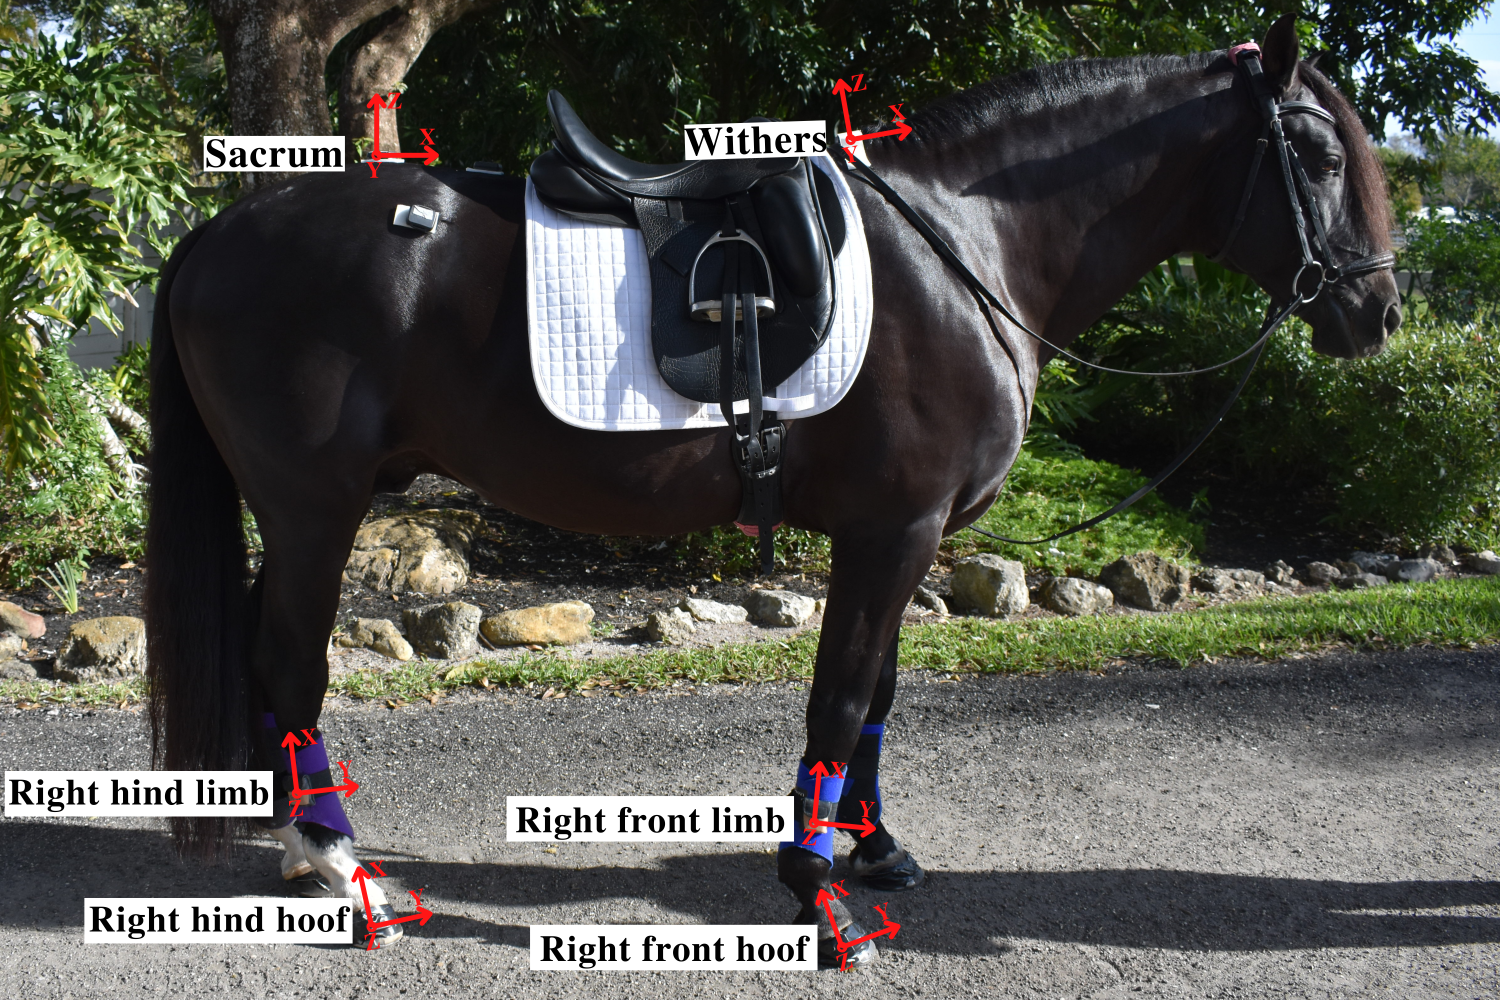
\includegraphics[width=.95\linewidth]{chapters/Step/figures/horse_step.png}
\caption{\gls{imu}s locations and orientations on horse body}
\label{horse}
\end{figure}

The three axes of rotation for the sacrum, withers, and poll \gls{imu}s were x,y, and z (Figure \ref{horse}), which were defined in the order as longitudinal axis, mediolateral axis, and vertical axis. For limbs and hooves, x, y, and z axes were aligned to the cannon and external hoof wall, (longitudinally), retraction/protraction angle axis, and abduction/adduction angle axis, respectively \cite{456}. 

The ethical permissions for the measurement and data collection were given by University of Central Lancashire (ethics code: STEMH961) and University of Kentucky (ethics code: 2019-3150).

Using the video footage of the measurements, the gaits (walk, trot, canter, piaffe, and passage) were labeled per stride. It should be noted that all the measurements were not gait-labeled. To study the performance of the estimation model independent of gait and to increase the size of the data, the part of the measurements that were not labeled was used for model development and evaluation. These measurements are comprised of strides during walk, trot, canter, piaffe, and passage. Hereafter, the part of the data that was not labeled is designated as “unlabeled” in this chapter.

In the literature, various methods labeled the hoof on/off moments by using the signals extracted from a hoof-mounted \gls{imu}. In a number of studies, the moment that the hoof-\gls{imu} acceleration signal (vertical acceleration) changes abruptly was labeled as “hoof-on moment” \cite{barstow_2018_does, hernlund_2013_hoof, chateau_2009_effects, holdendouilly_2013_equine, alsaaod_2017_the, witte_2004_determination, starke_2012_accuracy,adsd1}. In a few numbers of these studies, the final abrupt peak before silence on the signal pattern was labeled as “hoof-off moment” \cite{alsaaod_2017_the, witte_2004_determination, starke_2012_accuracy}. In this chapter, we used both methods for detecting and labeling the hoof on/off moments. 
	
The position of \gls{imu} on the hoof was different between the studies. For example, in one study, the \gls{imu} was mounted on the dorsal surface of the hoof, and in another study, the \gls{imu} was attached to the hoof lateral wall, while both studies used the vertical acceleration signal to detect the hoof-on and hoof-off moments. In Figure \ref{signals}, it is demonstrated that the x-axis (in the global coordinate system) of acceleration can present abrupt deceleration and accelerations, however, the x-axis of hoof-mounted \gls{imu} was not aligned exactly vertical, as shown in Figure \ref{hoof}. To cancel out the effect of different \gls{imu} positions and orientations on the hoof-mounted \gls{imu} alignment, the root of the sum of the squares (or Euclidean norm) of preprocessed tri-axial acceleration signals was calculated \cite{tijssen_2020_automatic,tijssen_2020_automatic_2}. Euclidean norm resulted in a unidirectional acceleration signal, which was plotted in time for identifying and labeling the moments observationally (bottom plot of Figure \ref{signals}). 
	
	\begin{figure}[tb]
\centering
\includegraphics[width=.65\linewidth]{chapters/Step/figures/signals_Step.png}
\caption{Acceleration signals extracted from right front hoof-mounted \gls{imu}. The signals were aligned on the global coordinate system. The green circles are the hoof-off moments and the red circles are the hoof-on moments. The plots were time-synchronized. The vertical and horizontal axes of the plots are in acceleration $m/s^{2}$ and timesteps (each timestep = 5 milliseconds), respectively}
\label{signals}
\end{figure}

\begin{figure}[htbp]
\centering
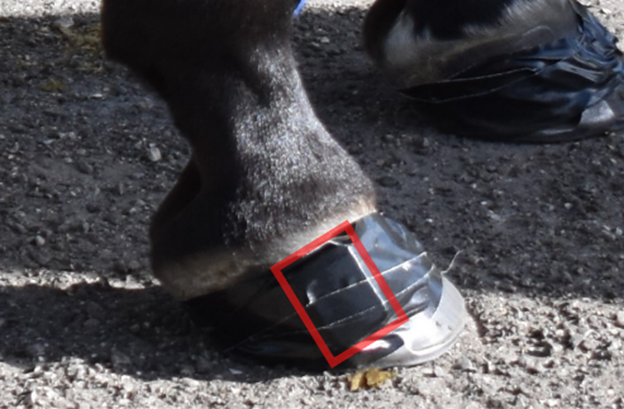
\includegraphics[width=.5\linewidth]{chapters/Step/figures/hoof_step.png}
\caption{The placement of \gls{imu} on the wall of the right front hoof, indicated by the red box}
\label{hoof}
\end{figure}
	
Each timestep was labeled (according to the Euclidean acceleration signal obtained from hoof-\gls{imu}) as "1" if it was a hoof-on moment or "0" if it was not a hoof-on moment. Therefore, for each hoof, a label signal was produced consisting of zeros and ones (in the form of a square wave signal).
	
\subsection{Feature selection and dataset preparation}

	Eight signals were from each \gls{imu} extracted. The extracted signals consisted of three acceleration signals, three angular velocity signals, one Euclidean norm of the three acceleration signals, and one Euclidean norm of the three angular velocity signals. All the eight signals and the label signal were time-synchronized with an accuracy smaller than 100 milliseconds. Therefore, the goal of each model is to estimate the label signal using the eight-dimensional input derived from one of the \gls{imu}s.
	
The models were trained using a ten-fold cross-validation method to prevent overfitting. The dataset from all subjects and gaits on each fold was split into approximately 90 percent training dataset and 10 percent testing dataset. More specifically, on each split, the data from at least two horses were on the testing dataset, and the remaining were on the training dataset. After each split, the training dataset was normalized using Z-score \cite{clarkcarter_2014_z}. The Z-score is defined as:

\begin{equation}\label{eq:zscore}
Z = \frac{X - \mu}{\sigma}
\end{equation}

where X is the signal, and $\mu$ and $\sigma$ are the mean value and the standard deviation of the signal, respectively. The testing set was normalized afterward using the parameters from the Z-score. The Z-score parameters were calculated using the training dataset instead of the whole dataset (training and testing datasets) to remove the normalization bias from the testing data.

For each "1" in the label signal, 127 time-synchronized windows (256-timestep window size) were created from each eight input signal and label signal. A clarification is provided by assuming that a hoof-on moment ("1" in label signal) occurred at timestep n. If $\left\{t\in\mathbb{N},1<t<127\right\}$, the windows for each n were in the range of $(n-2\times t,n+2\times (127-t)+1)$, which results in 127 windows. This sliding window for each "1" was applied to adapt the model to different locations of the moment within a window. It should be noted that all the windows used for training and testing datasets contained at least one hoof-on or hoof-off moment.

\subsection{Loss function}

Because of the scarcity of hoof-on and hoof-off moments compared to the non-moments, a loss function was required to focus the model on moments estimation since the goal of an estimation model is to minimize the loss. In this case, the loss function should be designed with the purpose of higher value returns from the model when it estimates the moment as "0" instead of "1", known as penalization of the model's incorrect estimation \cite{aurelio_2019_learning}. Hence, a weighted binary cross-entropy loss function has been defined as follows \cite{ho_2020_the},

\begin{equation}
L(y,\hat{y})=-(Wy\log(\hat{y})+(1-y)\log(1-\hat{y}))
\end{equation}

\noindent where $y$ and $\hat{y}$ are the true and predicted output, respectively. $W$ is the weight, which represents the extent of penalizing the incorrect model estimation. In the binary cross-entropy loss function, the logarithmic function is used instead of the linear form, which was 

\begin{equation}
L(y,\hat{y})=y\hat{y}+(1-y)(1-\hat{y})
\end{equation}

\noindent to heavily penalize the model estimations that are confidently wrong. For instance, if $y = 1$ and $\hat{y}\sim 0$, the first part of the binary cross-entropy function, $y\log(y)$, outputs a very high value according to Figure \ref{log_step}, while the second part, $(1-y)\log(1-y)$, yields a value of zero (or near zero). Using a weighted loss function, the first part is multiplied by $W$, which yields a bigger value for the loss function when there is a wrong prediction for events (when $y = 1$). Hence, the model tries to optimize the loss function, particularly during events. In contrast, if we do not use logarithm in the loss function, the value of the loss function would become zero (or near zero) and the model had been optimized already. In the current study, we considered $W$ as a hyperparameter and searched for the best model performance with $W$ values between 50,100, and 200.

\begin{figure}[htbp]
\centering
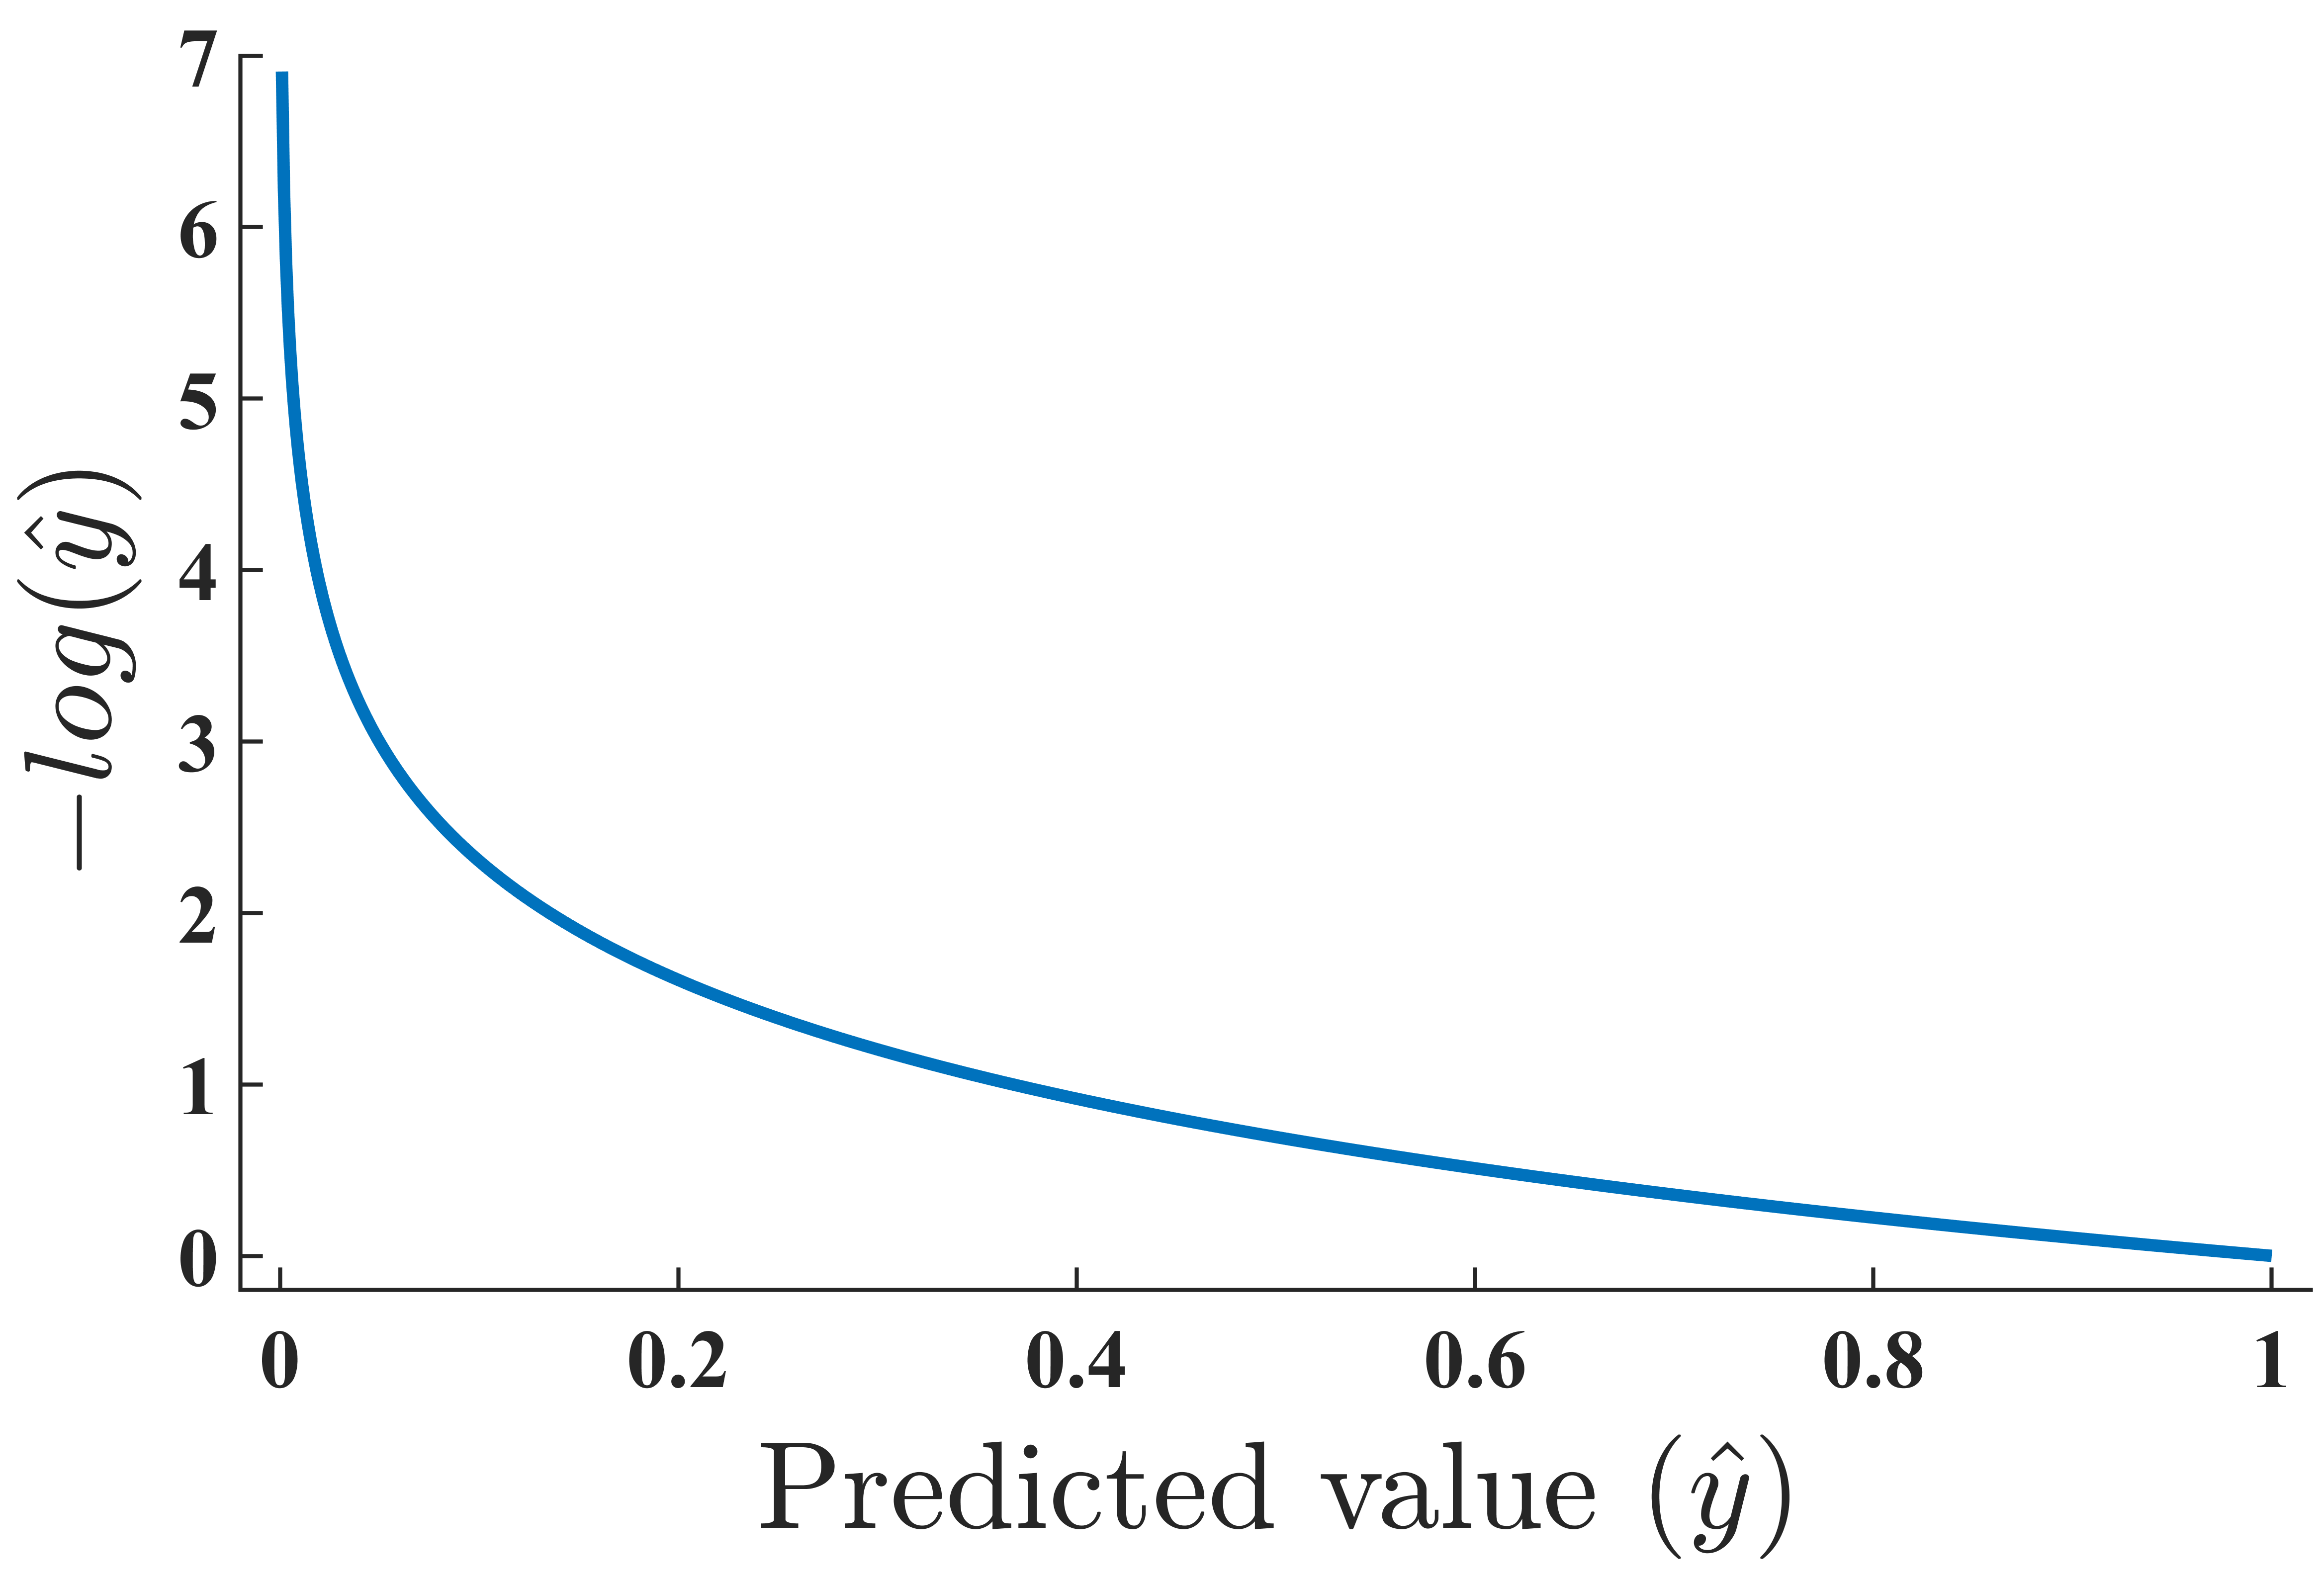
\includegraphics[width=.6\linewidth]{chapters/Step/figures/20210330_log.png}
\caption{The logarithm graph}
\label{log_step}
\end{figure}


\subsection{Model training, testing, and optimization}
Single-layer 256 units \gls{rnn} models with \gls{lstm} architecture (\gls{rnn}-\gls{lstm}) were implemented on the training dataset extracted from each \gls{imu} separately to optimize the customized loss function. In total, eight \gls{rnn}-\gls{lstm} models were trained and optimized, which were one hoof-on and one hoof-off moments estimation models for each \gls{imu}. \gls{rnn} was chosen since we tried to model and estimate time-series data. In addition, we selected \gls{lstm} as the architecture since it solves the \gls{rnn} issue of vanishing gradient during training time-series models. In total, the model received the eight-dimension input in 256-timestep windows (8×256), followed by a dropout layer, and a fully connected layer to the one-dimensional label signal as the output, as shown in Figure \ref{system_step}.

Since the estimation approach in this study is regression and not classification, the predicted outputs would not be binary; instead, they were signals. Therefore, we detected the maximum peak of each window (global maxima) in the output signal and counted it as the predicted event. Then, for evaluating the models, the time difference (in milliseconds and timesteps) between the true moment from the label signal and the maximum peak in the model output was calculated as the model error. The estimation errors were presented as the accuracy (mean of errors) and precision (standard deviation of errors) of the models.

In addition to $W$ as a hyperparameter, batch size (= 16, 32, 64, 128), learning rate (= 0.01, 0.05, 0.001, 0.005, 0.0001), and dropout rate (= 0.2, 0.4, 0.6) were also tuned for each model with the purpose that the model achieve the best overall accuracy and precision.

\subsection{Comparison of results with state of the art}
The best performing method (algorithm number 3) of \cite{adsd1} was selected to compare estimation performance results between the current study and state-of-the-art methods. The selected method was based on the inputs from limb-mounted \gls{imu} signals. Therefore, it was only implemented on the dataset (combined training and testing datasets) extracted from the right front and the right hind limb \gls{imu}s. Then, the errors were calculated as the same as discussed for our models and were compared with our results.

Matlab R2020a (MathWorks Inc., Natick, MA, USA) was used for data preprocessing, windowing, and state-of-the-art method calculations, while \gls{lstm} models were implemented, trained, and tested with Python 3.7 (Python Software Foundation, USA) (Keras 2.4.0 (https://keras.io/) and Tensorflow 2.4.0 as the backend).



